\iffalse
\let\negmedspace\undefined
\let\negthickspace\undefined
\documentclass[journal,12pt,twocolumn]{IEEEtran}
\usepackage{cite}
\usepackage{amsmath,amssymb,amsfonts,amsthm}
\usepackage{algorithmic}
\usepackage{graphicx}
\usepackage{textcomp}
\usepackage{xcolor}
\usepackage{txfonts}
\usepackage{listings}
\usepackage{enumitem}
\usepackage{mathtools}
\usepackage{gensymb}
\usepackage{comment}
\usepackage[breaklinks=true]{hyperref}
\usepackage{tkz-euclide}
\usepackage{listings}
\usepackage{gvv}
\def\inputGnumericTable{}
\usepackage[latin1]{inputenc}
\usepackage{color}
\usepackage{array}
\usepackage{longtable}
\usepackage{calc}
\usepackage{multirow}
\usepackage{hhline}
\usepackage{ifthen}
\usepackage{lscape}

\newtheorem{theorem}{Theorem}[section]
\newtheorem{problem}{Problem}
\newtheorem{proposition}{Proposition}[section]
\newtheorem{lemma}{Lemma}[section]
\newtheorem{corollary}[theorem]{Corollary}
\newtheorem{example}{Example}[section]
\newtheorem{definition}[problem]{Definition}
\newcommand{\BEQA}{\begin{eqnarray}}
\newcommand{\EEQA}{\end{eqnarray}}
\newcommand{\define}{\stackrel{\triangle}{=}}
\theoremstyle{remark}
\newtheorem{rem}{Remark}
\begin{document}

\bibliographystyle{IEEEtran}
\vspace{3cm}

\title{NCERT Discrete 11.9.3 -26}
\author{EE23BTECH11057 - Shakunaveti Sai Sri Ram Varun$^{}$% &lt;-this % stops a space
}
\maketitle
\newpage
\bigskip
\vspace{2cm}
\textbf{Question: }
Insert two numbers between 3 and 81 so that the resulting sequence is G.P.\\
\textbf{Solution}:
\fi
\begin{table}[htbp] 
\centering
\begin{tabular}{|c|c|c|}
    \hline
    \textbf{Parameter} & \textbf{Description} & \textbf{Value} \\
    \hline
    $x\brak{0}$ & First term of G.P. & 3 \\
    \hline
    $x\brak{3}$ & Fourth term of G.P. & 81 \\
    \hline
    $r$ & common ratio of G.P. & r \\
    \hline
\end{tabular}



\caption{input values}
\label{tab: Table 11.9.3.26.15}
\end{table}
\begin{enumerate}
\item 
\begin{align}
x\brak{n}=x\brak{0}r^{n}
\end{align}
from the values in \tabref{tab: Table 11.9.3.26.15}
\begin{align}
%x(0)&=3\\
%x(3)&=81\\
\frac{x\brak{0}r^3}{x\brak{0}}&=27\\
r&=3
\end{align}
$ \therefore $ Required numbers are 9 and 27.
\item 
\begin{align}
x\brak{n} &= 3^{n+1}u\brak{n} \label{eq:11.9.3.26.1}\\
X\brak{z} &= \frac{3}{1-3z^{-1}} \quad |z|>3 \label{eq:11.9.3.26.2}
\end{align}
\begin{figure}[h!]
    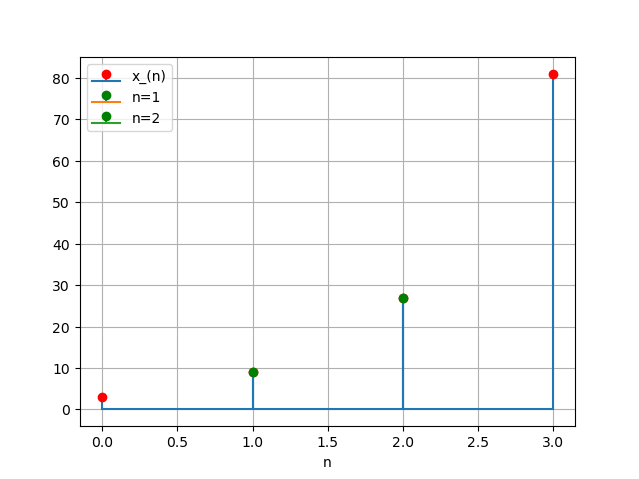
\includegraphics[width = \columnwidth]{ncert-maths/11/9/3/26/figs/Figure_1.png}
    \caption{Graph of $ x\brak{n}$ }
    \label{fig: 11.9.3.26.17}
\end{figure}
\end{enumerate}

